\documentclass[]{scrartcl}
\usepackage[T1]{fontenc}
%\usepackage{lmodern}
\usepackage{fourier}
\usepackage{epstopdf}
\usepackage{mathtools}
\usepackage{fancyhdr}
\usepackage{caption}
\usepackage[margin=1in]{geometry}
\usepackage{slashbox}
\usepackage[utf8]{inputenc}
\usepackage[polish]{babel}														% English 
\usepackage{multirow}
\usepackage[protrusion=true,expansion=true]{microtype}					% Better typography
\usepackage[pdftex]{graphicx}	
\usepackage{amsmath,amsfonts,amsthm}										% Math packages
									% Enable pdflatex
\pagenumbering{gobble}
\usepackage{url}

%opening
%opening
\title{Metody symulacji \\ \normalsize{Testowanie generatorów liczb losowych \\ Temat II d}}
\date{} 

\author{ Rafał Skrzypiec \\ \normalsize{\text{263957}}\\}
	

\begin{document}
	
	\maketitle


\section*{Opis testu}



Do testowania generatorów liczb losowych ran3 oraz r250 wykorzystano test oparty na zjawisku błądzenia losowego na sieci trójkątnej. Wędrowniczek startuje z punktu (0,0) i po wykonaniu $L$ kroków kończy spacer w punkcie ($x$,$y$). Dokonując podziału płaszczyzny na 6 równych części, sprawdzamy, w której z nich wędrowniczek zakończył spacer.
Nasza hipoteza zakłada trajektoria cząstki startującej z początku układu współrzędnych powinna z jednakowym prawdopodobieństwem kończyć się w jednej z 6 części płaszczyzny. Aby sprawdzić jej prawdziwość przeprowadzimy test zgodności $\chi^2$.


\begin{figure}[!h]
	\centering
	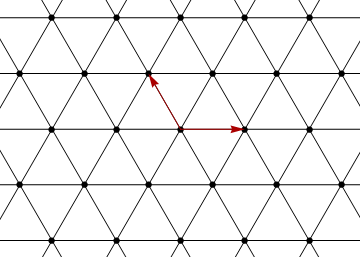
\includegraphics[width=0.5\linewidth]{hexagonal}
	\caption{Przykład sieci trójkątnej [1]}
\end{figure}

Biorąc pod uwagę fakt, że prawdopodobieństwo $p_i$ zakończenia spaceru w części $i$ wynosi $1/6$ możemy obliczyć wartość statystyki $\chi^2$ ze wzoru:

$$
V = \frac{6}{n}\;\; \sum_{i = 0}^{5}\;\left( n_i - \frac{n}{6}  \right)^2
$$

Wybierając poziom istotności na poziomie 0.02, dla przypadku z 5 stopniami swobody zbiór krytyczy wynosi [2]:
$$
\chi < \chi_{0.01} = 0.55 \;\;\;\;\; \text{lub} \;\;\;\;\; \chi > \chi_{0.99} = 15.09
$$


\clearpage

\section*{Metodyka}

Aby symulować ruch hipotetycznej cząstki wprowadziłem 6 wektorów, o które może zmienić położenie: $e_0 = (1,0)$,  $e_1 = (0.5, -\frac{\sqrt{3}}{2})$,  $e_2 = (-0.5, -\frac{\sqrt{3}}{2})$,  $e_3 = (-1,0)$,  $e_4 = (-0.5, \frac{\sqrt{3}}{2})$,  $e_5 = (0.5, \frac{\sqrt{3}}{2}) $

Następnie losowałem w $L$ krokach losowałem numery wektora sieciowego, zmieniając położenie wędrowniczka o wylosowany wektor. Całą płaszczyzną podzieliłem na 6 równych części oraz punkt (0,0) według zasad:

\begin{table}[h!]
	\centering
	\caption{Zdefiniowane obszary płaszczyzny}
	\begin{tabular}{|c| c|}
		\hline
		Obszar & Warunki \\ \hline
		0  & $x\geq0$ i $y>\frac{x}{\sqrt{3}}$   \\ \hline
		1  & $y\leq\frac{x}{\sqrt{3}}$ i $y > -\frac{x}{\sqrt{3}}$\\ \hline
		2  & $y\leq - \frac{x}{\sqrt{3}}$ i $x > 0$   \\ \hline
		3  & $x\leq 0 $ i $y < \frac{x}{\sqrt{3}}$  \\ \hline
		4  & $y \geq \frac{x}{\sqrt{3}}$  i $y < - \frac{x}{\sqrt{3}}$ \\ \hline
		5  & $y \geq -\frac{x}{\sqrt{3}}$  i $x < 0$ \\ \hline
	    6  & $y = 0 $  i  $x = 0$ \\ \hline
	\end{tabular}
\end{table}

Następnie zliczałem ilość zakończeń wędrówki po $L$ krokach w każdym z obszarów, zakończenie wędrówki w obszarze nr 6 powodowało powtórzenie spaceru.
 

\begin{figure}[!h]
	\centering
	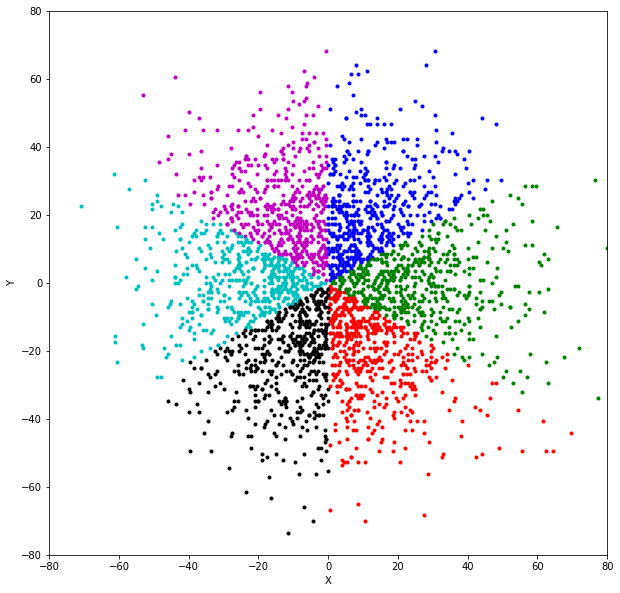
\includegraphics[width=0.8\linewidth]{hex_col}
	\caption{Płaszczyzna, na której zaznaczono 3000 punktów, w których wędrowniczek zakończył wędrówkę po 1000 kroków, każdy z kolorów odpowiada innemu obszarowi.}
\end{figure}



%\begin{figure}[!h]
%	\centering
%	\includegraphics[width=1\linewidth]{pera}
%	\caption{Prawdopodobieństwo wystąpienia klastra perkolacyjnego w zależności od koncetracji $c$.}
%\end{figure}

%\begin{figure}[h!]
%	\centering
%	\includegraphics[width=1\linewidth]{per3}
%	\caption{Prawdopodobieństwo wystąpienia klastra perkolacyjnego w zależności od koncetracji $c$, krzywe na wykresie to dopasowane do punktów wielomiany 4 stopnia.}
%\end{figure}

\clearpage

\section*{Wyniki}

Wykonano po 50 powtórzeń symulacji dla każdego z testów dla $10^5$ spacerów, które miały po 1000 kroków.

\begin{table}[h!]
	\centering
	\caption{Przykładowe wyniki symulacji dla $10^5$ spacerów}
	\begin{tabular}{|c| c| c| c| c| c|c| c|}
		\hline
		Generator & $n_0$ & $n_1$ & $n_2$ & $n_3$ & $n_4$ & $n_5$ & $V$\\ \hline
		 r250  & 17007 & 15812  & 16219 & 16625 & 17847& 16490 & 148.37\\ \hline
		ran3  &	16555  & 16495 & 16443 & 16958 & 17095 & 16454 & 24.33\\ \hline
	\end{tabular}
\end{table}




\begin{figure}[h!]
	\centering
	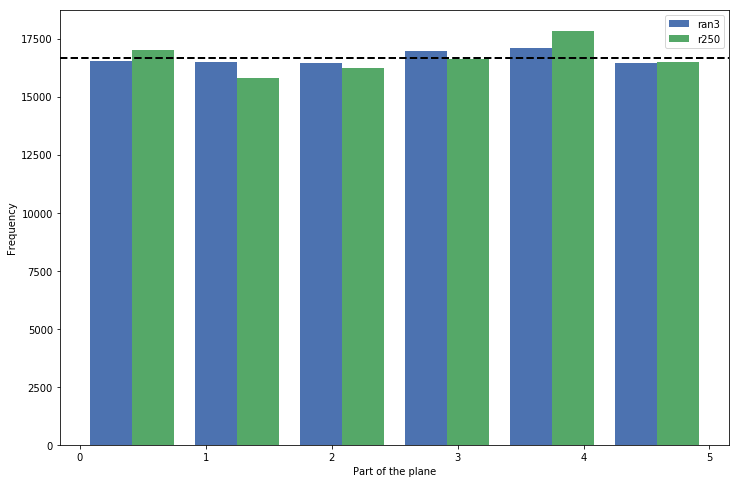
\includegraphics[width=1\linewidth]{hists}
	\caption{Przedstawienie wyników z powyższej tabeli na histogramie, przerywana linia zaznacza wartość $10^5$/6.}
\end{figure}


\begin{table}[h!]
	\centering
	\caption{Podsumowanie wyników symulacji}
	\begin{tabular}{|c|c| c| c|}
		\hline
		Generator & Ilość symulacji & "Srednie $V$ & Odchylenie standardowe $V$ \\ \hline
		r250  &50 &133.26 & 12.93 \\ \hline
		ran3  &50	&26.06  & 10.01\\ \hline
	\end{tabular}
\end{table}


\clearpage

\begin{figure}[h!]
	\centering
	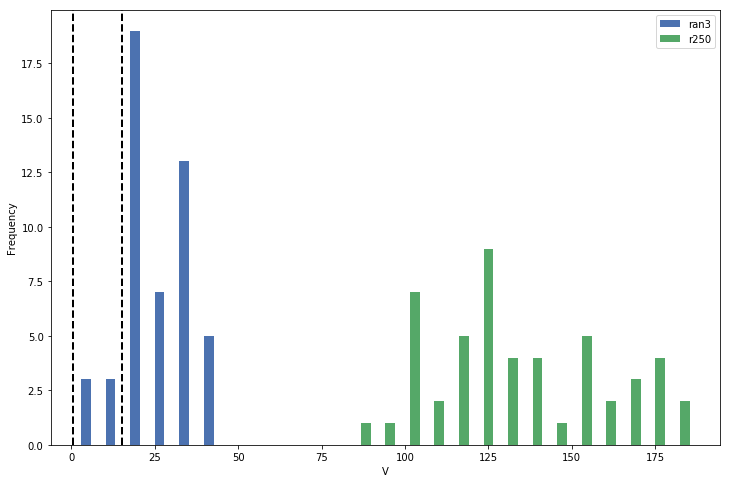
\includegraphics[width=1\linewidth]{hists1}
	\caption{Rozkład wartości $V$ dla 50 prób, każda po $10^5$ spacerów, dla generatorów ran3 i r250. Przerywane linie wyznaczają granice zbioru krytycznego.}
\end{figure}

\section*{Wnioski}

Analizując powyższe wyniki, zauważamy, że generator r250 nie zdaje testu zgodności $\chi^2$, średnia wartość statystyki $V$ wynosi 133.26, głęboko trafiając w zbiór krytyczny, który wynosi $V < 0.55 \;\;\; \text{lub} \;\;\;  V > 15.09$. Na 50 wykonanych testów, wszystkie z nich trafiły w zbiór krytyczny, co pozwala z całą pewnością stwierdzić, że generator r250 oparty na przesuwanym rejestrze nie jest dobrym generatorem liczb losowych.


Generator ran3 poradził sobie w teście nieco lepiej, jednak również nie zdał testu zgodności $\chi^2$, średnia wartość statystyki $V$, wynosi 26.06 i trafia w zbiór krytyczny, który wynosi $V < 0.55 \;\;\; \text{lub} \;\;\;\ V > 15.09$. Na 50 wykonanych testów, 44 z nich trafiły w zbiór krytyczny, pozwala to z całą pewnością stwierdzić, że generator Fibonacciego ran3 nie jest dobrym generatorem liczb losowych.

%ran3 generator fibonacciego p=55 q=24 m=$10^9$
%r250 generator oprarty na przesuwanym rejestrze p=250 q=103 

\begin{thebibliography}{99}

	\bibitem{1} \url{https://en.wikipedia.org/wiki/Hexagonal_lattice}
	 \label{1}		
	 	\bibitem{2} \url{http://www.itl.nist.gov/div898/handbook/eda/section3/eda3674.htm} \label{2}
	 	
	 	\bibitem{3} Wykład z Metod symulacji, prof. Czesław Oleksy \label{3}
\end{thebibliography}


\end{document}
http://astro.ia.uz.zgora.pl/~scikop/node/17
Wykład prof. Oleksego
https://en.wikipedia.org/wiki/Hexagonal_lattice
